\chapter{Background}
\label{ch:Background}

In this chapter, I present the concepts relevant to the subject of the thesis. First, I introduce the topic of MT and the type of architecture I focus on later in the work. Next, I outline the problem of ambiguity and bias in MT models.

% WSD (if I end up using it)

\section{Neural Machine Translation}
\label{sec:Background:NMT}

Machine Translation (MT) is the process of using computer technology to translate text from one natural language to another. This can be achieved using different paradigms. There are three main types of machine translation systems: Rule-based Machine Translation (RBMT), Statistical Machine Translation (SMT) and Neural Machine Translation (NMT). 

Conventional RBMT systems use pre-defined rules based on syntax, morphology and semantics, created by professional linguists. Since language is dynamic and evolves over time, these rules need frequent adaptation, which is costly. However, the key weakness of rule-based translation systems is that they require extensive lexicons and a large set of rules \parencite{SMT_book}. 

SMT systems, on the other hand, use a data-driven approach that utilizes statistical models derived from the analysis of bilingual and monolingual corpora. The quality of SMT output depends heavily on the size and quality of the corpora used to train the models. SMT’s general weakness is that it can only translate a phrase if it exists in the training dataset \parencite{SMT_book}.

Neural Machine Translation (NMT) is a subfield of SMT, which uses an artificial neural network to learn a statistical model for machine translation. Unlike traditional SMT systems, which require a pipeline of specialized components such as language model and translation model, NMT trains its statistical model end-to-end, mapping directly from an input source language to an output target language. NMT can recognize patterns in the training data to determine a context-based interpretation that can predict the likelihood of a sequence of words. Unlike SMT, NMT models are able to learn from each translation task and improve upon each subsequent translation. NMT models are more memory-efficient and also have a higher accuracy than SMT models, which makes them the appropriate choice for creating high-quality MT systems \parencite{NMT_book}.

% TODO: How in deep should I explain the Transformer and NMT?

\paragraph{Sequence-to-Sequence Modeling} 
The task of NMT is typically solved using Sequence-to-Sequence (Seq2Seq) modeling \parencite{seq2seq}. A Seq2Seq model has two parts: an encoder and a decoder. Both work separately and come together to form a large neural network model. This architecture has the ability to handle input and output sequences of variable length. A simplification of the architecture of NMT models can be seen in Fig. \ref{fig:seq2seq}. Firstly, each word in the input sentence is fed separately into the encoder to encode the source sentence into an internal fixed-length representation called the context vector. This context vector contains the meaning of the sentence. Secondly, the decoder decodes the fixed-length context vector and then predicts the output sequence.

\begin{figure}
  \centering
  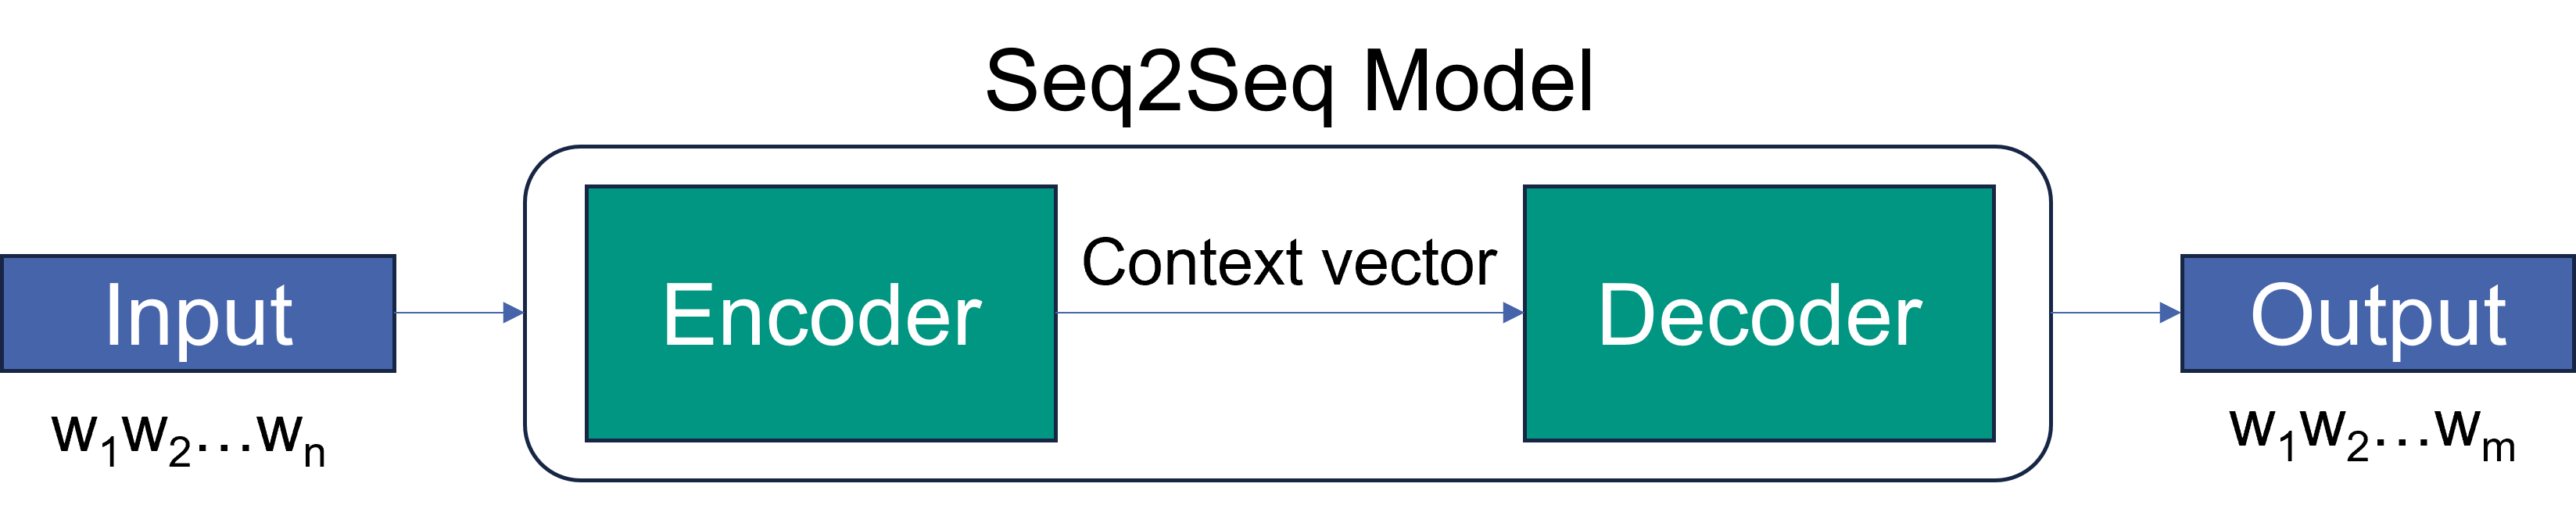
\includegraphics[scale=0.57]{figures/seq2seq.png}
  \caption{Sequence-to-Sequence Modeling}
  \label{fig:seq2seq}
\end{figure}

The original architecture consists of a pair of Recurrent Neural Networks (RNNs) in the roles of encoder and decoder. RNNs process the input sequence token by token, which prohibits parallelization and makes the training and inference slow, especially when processing longer sequences. Also, they suffer from vanishing or exploding gradients, which is inconvenient for effective training. One solution for these problems served Long Short-Term Memory (LSTM) networks, a type of RNN that has additional memory gates to regulate the flow of information through the network better \parencite{lstm}. Despite this, using a fixed-length context vector still incurs a bottleneck in the model. To alleviate this problem, the use of attention-based architectures for neural machine translation was explored \parencite{attention}. 

The attention mechanism allows the decoder to look at the source tokens that are relevant while generating the next token. Despite all these efforts, using RNN-based encoder and decoder still forces the network to handle input sequentially, which makes it difficult to handle long-range dependencies within the input and output sequences from memory. Hence, \cite{transformer} proposed the Transformer architecture, which replaces RNNs with self-attention layers in the Encoder-Decoder network. Since in this work I make use of models based on the Transformer, next I will introduce its basic principle and components.


\paragraph{Transformer Architecture} 
A Transformer is a Seq2Seq model, introduced by \cite{transformer}. An important feature of the Transformer architecture is its attention mechanism. The attention module looks at an input sequence and decides at each step which other parts of the sequence are important, differentially weighting the significance of each part of the input data. Like RNNs, Transformers are designed to handle sequential input data, such as natural language. However, unlike RNNs, Transformers can process the whole input sequence in parallel. The attention mechanism provides context for any position in the input sequence. This feature allows for more parallelization than RNNs and therefore reduces training times significantly \parencite{transformer}.

% Transformer Components
The Transformer architecture as presented in the original paper by \cite{transformer} is depicted in Fig. \ref{fig:transformer}.
The input embedding layer converts the high-dimensional input sequence into a low-dimensional sequence of vectors to capture the meaning and context.
The positional encoding preserves the sequential order of words in the input sentence and can be thought of as the distance of one word to another word in a sequence. This relative position of the words in the sequence is needed since the words are passed in parallel, as opposed to RNNs, which process them in order.
Self-attention is the weighted sum of all other words in the input sequence for each word using similarity (dot product) and SoftMax to focus on the most relevant parts of the input for each element. The multi-head attention repeats self-attention multiple times based on how many encoder/decoder layers there are.

There are multiple encoder and decoder layers. 
Each encoder has one multi-head self-attention, which encodes the weight of the input words to each other. 
Each decoder has one masked multi-head self-attention and one multi-head attention. The masked multi-head self-attention ensures that only words coming before a word are compared to that word, which means it only attends to preceding words in the input sequence during the decoding process. Applying a mask forces the model to ignore future words and focus only on the preceding words during the attention computation. % The mask specifically sets the attention weights to a very large negative value for the positions that correspond to future words, effectively making those weights close to zero after applying the softmax function. 
The multi-head cross-attention module in the decoder compares output tokens to input tokens.
Both the encoder and the decoder have one feed-forward layer, as well as adding and normalizing of residuals at each stage after the attention layers.

The output from the decoder is a vector of length of the input tokens. This output is fed into a fully connected (linear) layer to map it to a set of output prediction and then converted into probability over possible words like multi-class classification using a SoftMax layer.

\begin{figure}
  \centering
  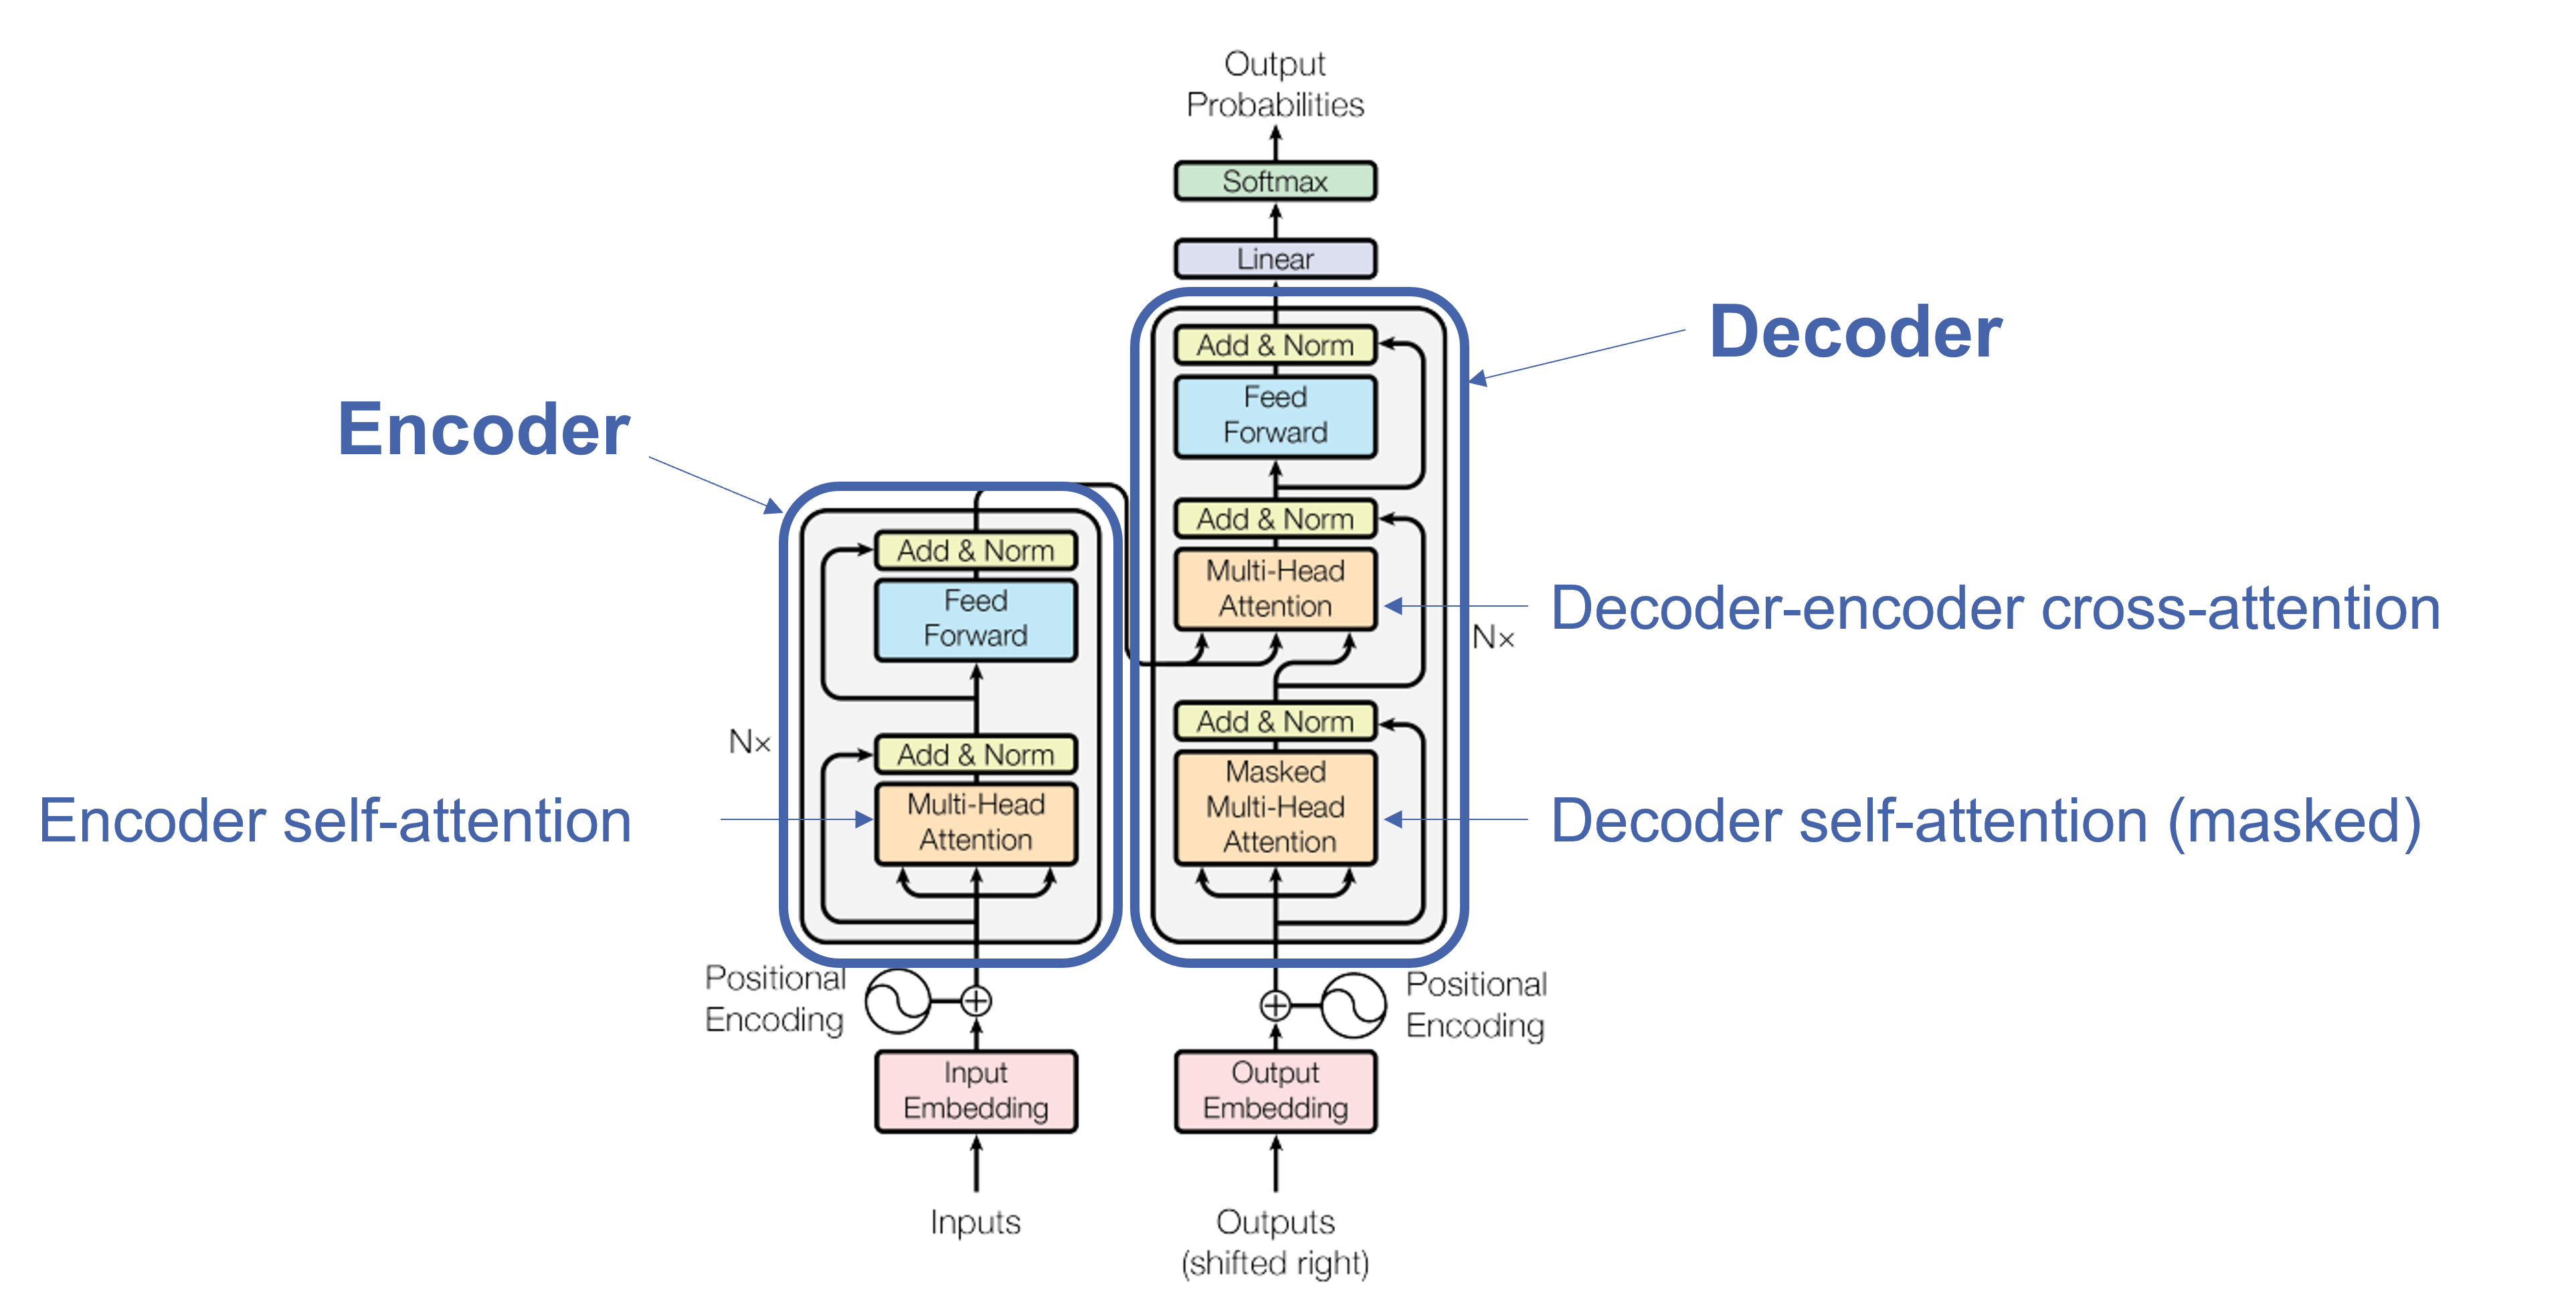
\includegraphics[scale=0.5]{figures/transformer.png}
  \caption{The Transformer Architecture}
  \label{fig:transformer}
\end{figure}


\section{Ambiguity and Bias in Machine Translation}
\label{sec:Background:Ambiguity_Bias}

% TODO
% - Definitions of bias and  ambiguity
% - Types of biases
% - Types of languages

Biases present in AI systems are an important problem stemming from cultural and historical issues present in the data from which models are learning. The developed systems in turn reinforce the present societal prejudices and old social norms, instead of mitigating them.

% “man is to computer programmer as woman is to homemaker” \parencite{bolukbasi2016man}

% For bias detection we need:
% - Challenge sets are artificially created usually small datasets that represent some gender-related issue, such as assigning the right pronoun to a specific role
% - Automatic evaluation methods needed, because the BLEU score, normally used for assessing the quality of translations, cannot judge on the occurrence of bias
% WSD: technique in natural language processing (NLP), defined as the ability to determine which meaning of word is activated by the use of word in a particular context
% QE: method for predicting the quality of a given translation rather than assessing how similar it is to a reference segment, E.g. multiple beams in Beam search: low confidence = high confidence for error in translation

